\section{Snapshots at Different Phase Points}
The typical phase diagramme of a Lennard-Jones potential near the critical point can be found in Fig.~\ref{fig:LJPhases}.
\begin{figure}[h!]
	\centering
	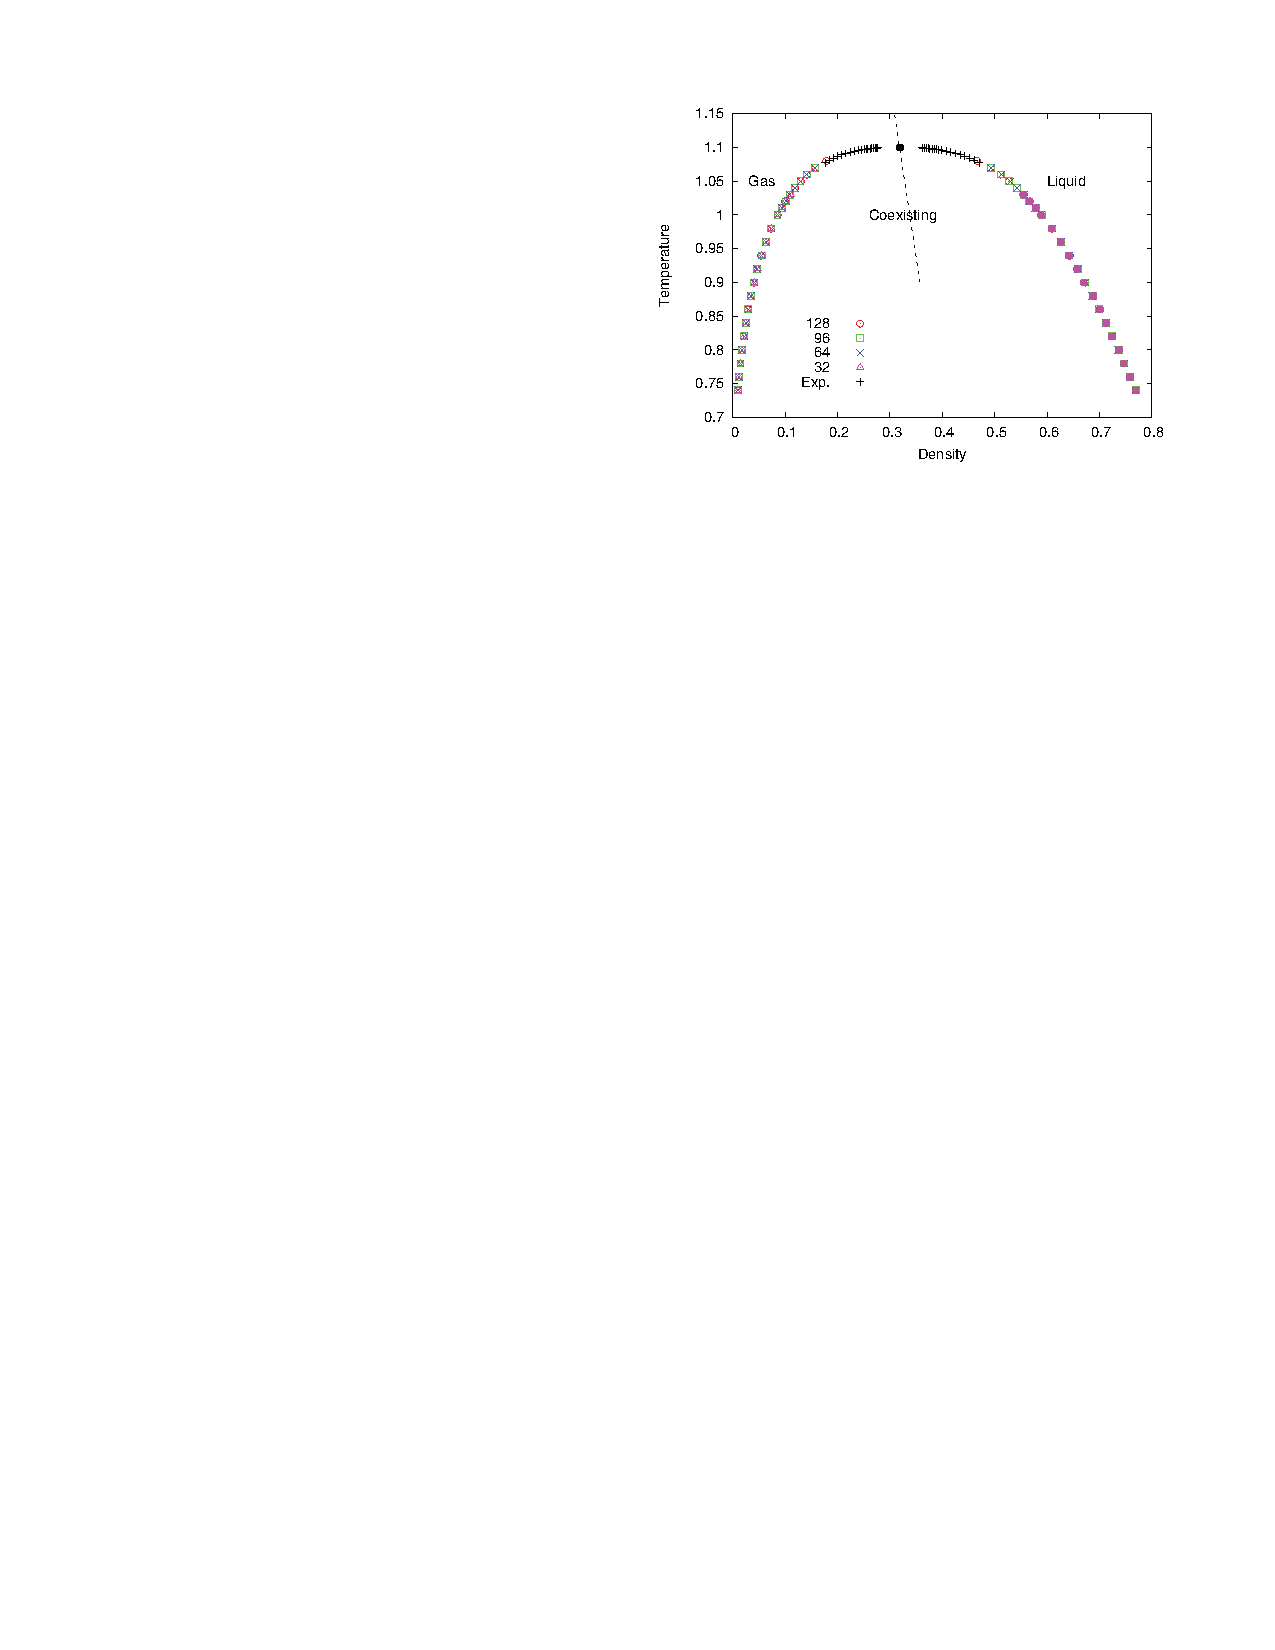
\includegraphics[width=0.6\textwidth]{LJPhases}
	\caption[LJ: Phase Diagramme]{The phase diagramme of a Lennard-Jones potential near the critical point~ZITIEREN!.}
\end{figure}
Hence after the system is in equilibrium, there can be found two phases - gaseous and liquid.
In principle, the function
\begin{align}
	\rho(z) = \frac{\rho_l - \rho_g}{2}\left(\tanh\left[(z_c-z)/lambda\right] + 1\right) + \rho_g
\end{align}
matches the density distribution and could be used to fit out the gaseous and liquid densities, respectively.
But for a simple and basic comparison, this reaches far beyond the scope of this work.
However, the next figure is an animation and shows snapshots of equilibrated states at different temperatures (Adobe Acrobat or similar PDF reader with java script support required).
\begin{figure}[h!]
	\centering
	\begin{minipage}[t]{\textwidth}
		\begin{minipage}[t]{0.4\textwidth}
			\centering
			\animategraphics[width=\textwidth,autoplay,loop,controls,buttonsize=1.2em]{0.5}{/animates/MCPhase}{1}{4}
		\end{minipage}
		\hspace{2cm}
		\begin{minipage}[t]{0.4\textwidth}
			\centering
			\animategraphics[width=\textwidth,autoplay,loop,controls,buttonsize=1.2em]{8}{/animates/MCPhaseSnapsT06}{0}{99}
		\end{minipage}
	\end{minipage}
	\caption[LJ Potential: Coexisting Phases at different temperatures]{Left: The coexisting phases mix together when the setting is close to the critical point.\\
	Right: 100 Frames show each step of an equilibrated state from the MC simulation.}
\end{figure}\\
For small densities and temperature, one can observe states resulting from the effects of PBC.
In explicit, these effects result in a droplet-liquid and a cylindrical-liquid phase, which can be seen in Fig.~\ref{fig:PBCPhases}.
\begin{figure}[ht]
	\centering
	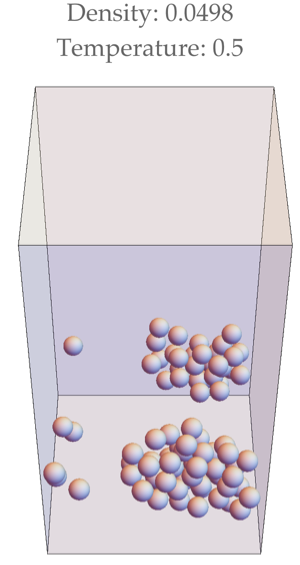
\includegraphics[width=0.3\textwidth]{MCDroplet}
	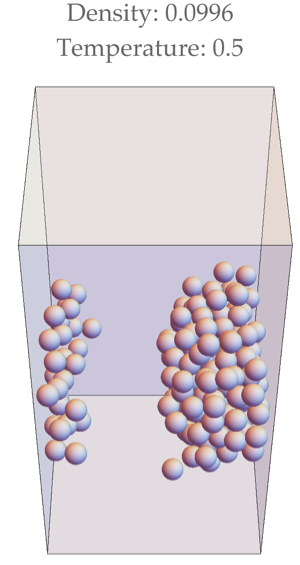
\includegraphics[width=0.3\textwidth]{MCCylinder}
	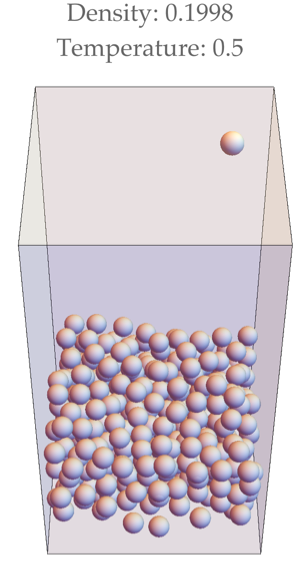
\includegraphics[width=0.3\textwidth]{MCCuboid}
	\caption[PBC: Phases Caused from Boundary Effects]{The phases shown above are caused from boundary effects.}
\end{figure}\\
Apart from side effects of PBC, perfect droplets are difficult to implement in a simulation, hence PBC are used to analyse droplet specifics e.g. surface tension.
